\section{Evaluation framework}\label{sec:software}

The current Neural Architecture Search (NAS) solutions lack a crucial element: an open-source framework for reproducibility and further research. Specifically for NAS with reinforcement learning, it would be desirable to build on a programming interface that allows researchers to explore the effect of different algorithms on the same NAS environment. In an attempt to fill this gap, we have developed the \textsc{nasgym}\footnote{Source code available at: github.com/gomerudo/nas-env}, a python OpenAI Gym~\citep{openaigym} environment that can jointly be used with all the reinforcement learning algorithms exposed in the OpenAI baselines~\citep{openaibaselines}. 

We make use of the object-oriented paradigm to abstract the most essential elements of NAS as a reinforcement learning problem, resulting in a system that can be extended to perform new experiments, as displayed in Figure~\ref{fig:software:architecture}. Although the defaults in the \textsc{nasgym} are the elements in our methodology, the system allows us to easily modify the key components, such as the performance estimation strategy, the action space, or the Neural Structure Code space. We also provide an interface to use a database of experiments that can help to store previously computed rewards, thus reducing the computation time of future trials. All the deep learning components are built with TensorFlow v1.12~\citep{tensorflow}.



\begin{figure}[ht]
\begin{center}
\begin{tikzpicture}

% definitions
\tikzstyle{boxA} = [rectangle, dashed, minimum width=2cm, minimum height=1cm, text centered, draw=black, fill=gray!0]
\tikzstyle{boxempty} = [rectangle, minimum height=1cm, text width=3cm, text centered, fill=gray!0]



\tikzstyle{arrow} = [->,>=stealth]


% box top
\draw (-4, 0) -- (-4, -4); % left
\draw (-4, 0) -- (-3, 0); % topA
\node at (-2.2, 0){\textsc{nasgym}}; % Label
\draw (-1.35, 0) -- (5, 0); % topB
\draw (-4, -4) -- (5, -4); % bottom
\draw (5, 0) -- (5, -4); % right


\node (nasenv) [boxA] at (0.75, -1) {\small \textsc{DefaultNasEnvironment}};

\node (datahandler) [boxA, below of=nasenv, yshift=-1cm, xshift=-2cm] {\small \textsc{DatasetHandler}};

\node (dbexperiments) [boxA, below of=nasenv, yshift=-1cm, xshift=2cm] {\small \textsc{DbInterface}};





\node (nscdef) [boxempty, left of=nasenv, xshift=-6cm] {\faFileCodeO \\ \small NSC \\definition file};

\node (config) [boxempty, below of=nscdef, yshift=-1cm] {\faFileCodeO \\ \small Hyper-parameters values};

\node (tfrecords) [boxempty, below of=datahandler, yshift=-1cm] {\faFilesO \\ \small TFRecords files};

\node (db) [boxempty, below of=dbexperiments, yshift=-1.2cm] {\faDatabase \\ \small Database of \\ experiments};


\draw [arrow] (nscdef) -- (nasenv);
\draw [arrow] (config) -- (nasenv.west);
\draw [arrow] (tfrecords) -- (datahandler);
\draw [arrow] (db) -- (dbexperiments);


\end{tikzpicture}
\caption{An sketch of the system built to perform our research. The \textsc{nasgym} package contains a default NAS environment whose states and actions are designed according to the Neural Structure Code (NCS) space defined in a \textit{.yml} file. The hyperparameters for all the machine learning components are defined in a \textit{.ini} file. Internally, the environment makes use of a dataset handler that reads TFRecords files and sends them as inputs to the neural architectures. A simple database of experiments is used to store experiments in a local file, although the logic can be easily be extended to support a more robust database system.}
\label{fig:software:architecture}
\end{center}
\end{figure}

Additionally to the \textsc{nasgym}, we implement the meta version of the A2C algorithm on top of the OpenAI baselines\footnote{Source code available at: github.com/gomerudo/openai-baselines}. We believe that this software engineering effort will help to compare, reproduce, and develop future research in NAS.
